% Options for packages loaded elsewhere
\PassOptionsToPackage{unicode}{hyperref}
\PassOptionsToPackage{hyphens}{url}
%
\documentclass[
]{article}
\usepackage{amsmath,amssymb}
\usepackage{iftex}
\ifPDFTeX
  \usepackage[T1]{fontenc}
  \usepackage[utf8]{inputenc}
  \usepackage{textcomp} % provide euro and other symbols
\else % if luatex or xetex
  \usepackage{unicode-math} % this also loads fontspec
  \defaultfontfeatures{Scale=MatchLowercase}
  \defaultfontfeatures[\rmfamily]{Ligatures=TeX,Scale=1}
\fi
\usepackage{lmodern}
\ifPDFTeX\else
  % xetex/luatex font selection
\fi
% Use upquote if available, for straight quotes in verbatim environments
\IfFileExists{upquote.sty}{\usepackage{upquote}}{}
\IfFileExists{microtype.sty}{% use microtype if available
  \usepackage[]{microtype}
  \UseMicrotypeSet[protrusion]{basicmath} % disable protrusion for tt fonts
}{}
\makeatletter
\@ifundefined{KOMAClassName}{% if non-KOMA class
  \IfFileExists{parskip.sty}{%
    \usepackage{parskip}
  }{% else
    \setlength{\parindent}{0pt}
    \setlength{\parskip}{6pt plus 2pt minus 1pt}}
}{% if KOMA class
  \KOMAoptions{parskip=half}}
\makeatother
\usepackage{xcolor}
\usepackage[margin=1in]{geometry}
\usepackage{color}
\usepackage{fancyvrb}
\newcommand{\VerbBar}{|}
\newcommand{\VERB}{\Verb[commandchars=\\\{\}]}
\DefineVerbatimEnvironment{Highlighting}{Verbatim}{commandchars=\\\{\}}
% Add ',fontsize=\small' for more characters per line
\usepackage{framed}
\definecolor{shadecolor}{RGB}{248,248,248}
\newenvironment{Shaded}{\begin{snugshade}}{\end{snugshade}}
\newcommand{\AlertTok}[1]{\textcolor[rgb]{0.94,0.16,0.16}{#1}}
\newcommand{\AnnotationTok}[1]{\textcolor[rgb]{0.56,0.35,0.01}{\textbf{\textit{#1}}}}
\newcommand{\AttributeTok}[1]{\textcolor[rgb]{0.13,0.29,0.53}{#1}}
\newcommand{\BaseNTok}[1]{\textcolor[rgb]{0.00,0.00,0.81}{#1}}
\newcommand{\BuiltInTok}[1]{#1}
\newcommand{\CharTok}[1]{\textcolor[rgb]{0.31,0.60,0.02}{#1}}
\newcommand{\CommentTok}[1]{\textcolor[rgb]{0.56,0.35,0.01}{\textit{#1}}}
\newcommand{\CommentVarTok}[1]{\textcolor[rgb]{0.56,0.35,0.01}{\textbf{\textit{#1}}}}
\newcommand{\ConstantTok}[1]{\textcolor[rgb]{0.56,0.35,0.01}{#1}}
\newcommand{\ControlFlowTok}[1]{\textcolor[rgb]{0.13,0.29,0.53}{\textbf{#1}}}
\newcommand{\DataTypeTok}[1]{\textcolor[rgb]{0.13,0.29,0.53}{#1}}
\newcommand{\DecValTok}[1]{\textcolor[rgb]{0.00,0.00,0.81}{#1}}
\newcommand{\DocumentationTok}[1]{\textcolor[rgb]{0.56,0.35,0.01}{\textbf{\textit{#1}}}}
\newcommand{\ErrorTok}[1]{\textcolor[rgb]{0.64,0.00,0.00}{\textbf{#1}}}
\newcommand{\ExtensionTok}[1]{#1}
\newcommand{\FloatTok}[1]{\textcolor[rgb]{0.00,0.00,0.81}{#1}}
\newcommand{\FunctionTok}[1]{\textcolor[rgb]{0.13,0.29,0.53}{\textbf{#1}}}
\newcommand{\ImportTok}[1]{#1}
\newcommand{\InformationTok}[1]{\textcolor[rgb]{0.56,0.35,0.01}{\textbf{\textit{#1}}}}
\newcommand{\KeywordTok}[1]{\textcolor[rgb]{0.13,0.29,0.53}{\textbf{#1}}}
\newcommand{\NormalTok}[1]{#1}
\newcommand{\OperatorTok}[1]{\textcolor[rgb]{0.81,0.36,0.00}{\textbf{#1}}}
\newcommand{\OtherTok}[1]{\textcolor[rgb]{0.56,0.35,0.01}{#1}}
\newcommand{\PreprocessorTok}[1]{\textcolor[rgb]{0.56,0.35,0.01}{\textit{#1}}}
\newcommand{\RegionMarkerTok}[1]{#1}
\newcommand{\SpecialCharTok}[1]{\textcolor[rgb]{0.81,0.36,0.00}{\textbf{#1}}}
\newcommand{\SpecialStringTok}[1]{\textcolor[rgb]{0.31,0.60,0.02}{#1}}
\newcommand{\StringTok}[1]{\textcolor[rgb]{0.31,0.60,0.02}{#1}}
\newcommand{\VariableTok}[1]{\textcolor[rgb]{0.00,0.00,0.00}{#1}}
\newcommand{\VerbatimStringTok}[1]{\textcolor[rgb]{0.31,0.60,0.02}{#1}}
\newcommand{\WarningTok}[1]{\textcolor[rgb]{0.56,0.35,0.01}{\textbf{\textit{#1}}}}
\usepackage{graphicx}
\makeatletter
\newsavebox\pandoc@box
\newcommand*\pandocbounded[1]{% scales image to fit in text height/width
  \sbox\pandoc@box{#1}%
  \Gscale@div\@tempa{\textheight}{\dimexpr\ht\pandoc@box+\dp\pandoc@box\relax}%
  \Gscale@div\@tempb{\linewidth}{\wd\pandoc@box}%
  \ifdim\@tempb\p@<\@tempa\p@\let\@tempa\@tempb\fi% select the smaller of both
  \ifdim\@tempa\p@<\p@\scalebox{\@tempa}{\usebox\pandoc@box}%
  \else\usebox{\pandoc@box}%
  \fi%
}
% Set default figure placement to htbp
\def\fps@figure{htbp}
\makeatother
\setlength{\emergencystretch}{3em} % prevent overfull lines
\providecommand{\tightlist}{%
  \setlength{\itemsep}{0pt}\setlength{\parskip}{0pt}}
\setcounter{secnumdepth}{5}
\setcounter{section}{-1}
\usepackage{fvextra}
\DefineVerbatimEnvironment{Highlighting}{Verbatim}{
  showspaces = false,
  showtabs = false,
  breaklines,
  commandchars=\\\{\}

\usepackage{bookmark}
\IfFileExists{xurl.sty}{\usepackage{xurl}}{} % add URL line breaks if available
\urlstyle{same}
\hypersetup{
  pdftitle={QRM II Graded Assignment (2), Period 1 2025},
  pdfauthor={Group 21 - Carlijn Calori, Julia Koeleman, Marit Springer \& Collin Veenstra},
  hidelinks,
  pdfcreator={LaTeX via pandoc}}

\title{QRM II Graded Assignment (2), Period 1 2025}
\usepackage{etoolbox}
\makeatletter
\providecommand{\subtitle}[1]{% add subtitle to \maketitle
  \apptocmd{\@title}{\par {\large #1 \par}}{}{}
}
\makeatother
\subtitle{Material by Sjoerd van Alten and Klervie Toczé}
\author{Group 21 - Carlijn Calori, Julia Koeleman, Marit Springer \&
Collin Veenstra}
\date{25-09-2025}

\begin{document}
\maketitle

\section{Introduction}\label{introduction}

This assignment is to be completed in groups of 3-4. Further, all
students in your group need to be assigned to the same R tutorial group
(Friday's tutorial). You can sign yourself up for a group on Canvas.
Please do so
\textbf{before the start of your first R tutorial on Friday September 5th.}
You can use the Discussion Board in Canvas if you do not have a group
yet or if your group is incomplete.

The assignment has 5 parts, and each part corresponds to the course
material of that week (with the exclusion of week 6, for which there is
no R programming material).

You are supposed to hand in these assignments on Canvas at the following
dates:

\begin{itemize}
\tightlist
\item
  \textbf{Deadline 1} \emph{Thursday September 25th, at 23:59pm}: you
  are supposed to hand in weeks 1, 2, and 3 of this assignment. This
  will determine 18\% of your overall course grade
\item
  \textbf{Deadline 2} \emph{Thursday October 9th, at 23:59pm}: you are
  supposed to hand in weeks 4, and 5 of this assignment. This will
  determine 12\% of your overall course grade
\end{itemize}

The R tutorials (each Friday) will consist of two halves. During the
first half, you will discuss the tutorial exercises. These can be
downloaded separately from Canvas. During the second half, you can work
on this graded assignment within your own group. The purpose is that you
find out how to work with R for doing statistical analyses by yourself.
The tutorial exercises are meant to teach you basic commands to get you
started, but to answer the problem sets in this assignment, you might
need to research your own solutions, and use functions and commands not
described in the tutorial exercises. Learning how to solve your own
research problems is integral part of learning R. When you and your
group get stuck on how to approach an exercise, the hierarchy in finding
your way is as follows:

\begin{itemize}
\tightlist
\item
  use the concepts from the tutorial exercises;
\item
  use the cheat sheets available on Canvas;
\item
  use Google, YouTube, StackOverflow, or another website;
\item
  ask the teacher.
\end{itemize}

The use of generative AI is \textbf{not} permitted and may result in a
grade of 0. See the AI protocol in the course manual for details.

To answer the assignment, you can simply fill out this R markdown
document. There are designated places which you can fill with R code.
There are also designated spaces for you to answer each question. Often,
the structure of an answer will be as follows. First, you type the R
code in the designated box. This will show how you analyzed the data to
get the answer to the question. Below the box for the R code, you will
then summarize your answer to the question, i.e.~what are the
conclusions that you draw from the data analysis?

When handing in, you are supposed to submit this .Rmd file, and a
knitted version of this document. You can knit this document to pdf,
word, or html. Knitting to pdf requires you to have a .tex distribution
installed on your computer. Knitting to Word requires you to have Word
installed.

The exercises are designed such that you should be able to finish the
majority of them during the tutorial each week. If you are not able to
finish them fully during that time, you are expected to work on it in
your own time using the computers on campus or your own device. It is
best to meet as a group in-person when working together. If you want to
work remotely, github is a good platform to guarantee smooth
collaboration. Alternatively, you can email this .Rmd file back and
forth to one another as a group, but this is not recommended as it is
more cumbersome.

We encourage you to keep your code blocks, printing statements, and
final answers, as short as possible. In any case, there is a page limit
of 6 pages per week, which encompasses the total length of this document
which consists of the questions, your coding lines, and your answers.
When your answers to questions of the respective week exceed this page
limit, they will not be graded, resulting in zero points.

Each week consists of 1, 2, or 3 subquestions. The total amount of
points you can earn per week is 20 points.

\section{Week 1}\label{week-1}

\begin{enumerate}
\def\labelenumi{\arabic{enumi}.}
\tightlist
\item
  Find the dataset ``movies1.tsv'' on Canvas. Describe your data set:
  How many observations does it have. How many variables are there? How
  many subjects? What consists of a subject? \textbf{[4 points]}
\end{enumerate}

\begin{Shaded}
\begin{Highlighting}[]
\NormalTok{movies }\OtherTok{\textless{}{-}} \FunctionTok{read.table}\NormalTok{(}\StringTok{"movies1.tsv"}\NormalTok{, }\AttributeTok{header=}\ConstantTok{TRUE}\NormalTok{)}

\FunctionTok{head}\NormalTok{(movies)}
\end{Highlighting}
\end{Shaded}

\begin{verbatim}
##   index  budget
## 1  1773 2.7e+07
## 2  2540 1.5e+07
## 3  1174 4.0e+07
## 4  3262 0.0e+00
## 5  4324 0.0e+00
## 6   214 1.2e+08
##                                                                            keywords
## 1                                        fbi island serial killer series of murders
## 2                                 fire winter santa claus snow storm christmas tree
## 3 police sequel police officer brother-in-law brother-in-law relationship black men
## 4                  masseuse thanksgiving party romance mother daughter relationship
## 5                                                               christian film food
## 6                         u.s. air force grocery jamaican meteorologist rescue boat
##   original_language               title popularity release_date   revenue
## 1                en         Mindhunters  17.193659   2004-05-07  21148829
## 2                en             Krampus  31.565117   2015-11-26  61548707
## 3                en        Ride Along 2  25.136082   2016-01-14 124827316
## 4                en         Enough Said  14.969093   2013-09-18  25288872
## 5                en Faith Like Potatoes   0.147886   2006-10-27         0
## 6                en   The Perfect Storm  25.752118   2000-03-15 325756637
##   runtime vote_average vote_count    genre release_year release_month
## 1     106          6.3        333 Thriller         2004             5
## 2      98          5.9        584   Comedy         2015            11
## 3     102          6.1        555   Comedy         2016             1
## 4      93          6.6        348    Drama         2013             9
## 5      97          6.0          9    Drama         2006            10
## 6     130          6.2        597    Drama         2000             3
##   release_day         first_actor first_actor_gender director_first_name
## 1           7             LL Cool               <NA>               Renny
## 2          26          Adam Scott               male             Michael
## 3          14          Kevin Hart               male                 Tim
## 4          18 Julia Louis-Dreyfus             female              Nicole
## 5          27    Frank Rautenbach               male             Regardt
## 6          15      George Clooney               male            Wolfgang
##   director_gender
## 1            male
## 2            male
## 3            male
## 4          female
## 5            <NA>
## 6            male
\end{verbatim}

\begin{Shaded}
\begin{Highlighting}[]
\FunctionTok{ncol}\NormalTok{(movies)}
\end{Highlighting}
\end{Shaded}

\begin{verbatim}
## [1] 19
\end{verbatim}

\begin{Shaded}
\begin{Highlighting}[]
\FunctionTok{nrow}\NormalTok{(movies)}
\end{Highlighting}
\end{Shaded}

\begin{verbatim}
## [1] 505
\end{verbatim}

\textbf{Your Answer}

We conclude that the data set has 19 variables and 505 subjects. Every
subject consists of a unique movie.

\begin{enumerate}
\def\labelenumi{\arabic{enumi}.}
\setcounter{enumi}{1}
\tightlist
\item
  Which of the following types of variables are present in your data
  set? (i) nominal; (ii) ordinal; (iii); interval; (iv) ratio. If
  present, name one example of such a variable present in your data set.
  \textbf{[4 points]}
\end{enumerate}

\begin{Shaded}
\begin{Highlighting}[]
\CommentTok{\#WRITE YOUR CODE HERE}
\FunctionTok{str}\NormalTok{(movies)}
\end{Highlighting}
\end{Shaded}

\begin{verbatim}
## 'data.frame':    505 obs. of  19 variables:
##  $ index              : int  1773 2540 1174 3262 4324 214 1737 610 2738 963 ...
##  $ budget             : num  2.70e+07 1.50e+07 4.00e+07 0.00 0.00 1.20e+08 2.80e+07 7.00e+07 1.25e+07 4.00e+07 ...
##  $ keywords           : chr  "fbi island serial killer series of murders" "fire winter santa claus snow storm christmas tree" "police sequel police officer brother-in-law brother-in-law relationship black men" "masseuse thanksgiving party romance mother daughter relationship" ...
##  $ original_language  : chr  "en" "en" "en" "en" ...
##  $ title              : chr  "Mindhunters" "Krampus" "Ride Along 2" "Enough Said" ...
##  $ popularity         : num  17.194 31.565 25.136 14.969 0.148 ...
##  $ release_date       : chr  "2004-05-07" "2015-11-26" "2016-01-14" "2013-09-18" ...
##  $ revenue            : num  2.11e+07 6.15e+07 1.25e+08 2.53e+07 0.00 ...
##  $ runtime            : int  106 98 102 93 97 130 108 99 100 99 ...
##  $ vote_average       : num  6.3 5.9 6.1 6.6 6 6.2 5.5 4.4 6 6.2 ...
##  $ vote_count         : int  333 584 555 348 9 597 640 533 210 371 ...
##  $ genre              : chr  "Thriller" "Comedy" "Comedy" "Drama" ...
##  $ release_year       : int  2004 2015 2016 2013 2006 2000 2016 2014 2014 2009 ...
##  $ release_month      : int  5 11 1 9 10 3 2 1 2 9 ...
##  $ release_day        : int  7 26 14 18 27 15 4 10 14 29 ...
##  $ first_actor        : chr  "LL Cool" "Adam Scott" "Kevin Hart" "Julia Louis-Dreyfus" ...
##  $ first_actor_gender : chr  NA "male" "male" "female" ...
##  $ director_first_name: chr  "Renny" "Michael" "Tim" "Nicole" ...
##  $ director_gender    : chr  "male" "male" "male" "female" ...
\end{verbatim}

\textbf{Your Answer:}

Nominal: present, for example genre and title Ordinal: not present
Inverval: present, for example release\_year Ratio: present, for example
budget and revenue

\begin{enumerate}
\def\labelenumi{\arabic{enumi}.}
\setcounter{enumi}{2}
\tightlist
\item
  A movie studio wants to know which types of movies give maximal
  profit. Perform the following steps to provide the movie studio with
  an analysis which corresponds to their request:
\end{enumerate}

\begin{enumerate}
\def\labelenumi{\alph{enumi}.}
\tightlist
\item
  Create the variable profits as the revenue of a movie minus its
  budget. Report its mean, median, maximum, and minimum.
  \textbf{[2 points]}
\item
  Which movie has the highest profits in your data set and how much are
  these profits. Which movie has the lowest and how much are its
  profits? If multiple movies have the exact same highest or lowest
  profits, give only one example. \textbf{[2 points]}
\item
  Create a boxplot of the variable profits. Make sure it has an
  appropriate title, and appropriate titles and labels for the x- and
  y-axis. Give Q1, Q2, Q3, and Q4. What does this tell you about the
  nature of making money in the movies industry? \textbf{[2 points]}
\item
  Add a new variable to your data set the log of profits. When creating
  this variable, what happens to movies for which profits is zero or
  negative? What then happens when you calculate the mean of log of
  profits? \textbf{[2 points]}
\item
  For movies that have a profit of zero or less, replace log of profits
  with ``NA''. What is now the mean of log of profits? Create a boxplot
  for log of profits, again with an appropriate title, x- and y-axis
  labels. How does it compare to the boxplot you made under c.)?
  \textbf{[2 points]}
\item
  Create a scatterplot of with the runtime of movies on the x-axis and
  the average vote of movies on the y-axis. What do you conclude from
  the scatterplot? Are movies with a longer runtime considered worse or
  better by the audience, or does the audience not have a preference?
  Why do you think this is the case? \textbf{[2 points]}
\end{enumerate}

For each step, you should provide first all the code you used to answer
the question and then formulate an answer using full sentences.

\emph{Step a}

\begin{Shaded}
\begin{Highlighting}[]
\FunctionTok{library}\NormalTok{(tidyverse)}
\end{Highlighting}
\end{Shaded}

\begin{verbatim}
## -- Attaching core tidyverse packages ------------------------ tidyverse 2.0.0 --
## v dplyr     1.1.4     v readr     2.1.5
## v forcats   1.0.0     v stringr   1.5.1
## v ggplot2   3.5.2     v tibble    3.3.0
## v lubridate 1.9.4     v tidyr     1.3.1
## v purrr     1.0.4     
## -- Conflicts ------------------------------------------ tidyverse_conflicts() --
## x dplyr::filter() masks stats::filter()
## x dplyr::lag()    masks stats::lag()
## i Use the conflicted package (<http://conflicted.r-lib.org/>) to force all conflicts to become errors
\end{verbatim}

\begin{Shaded}
\begin{Highlighting}[]
\NormalTok{movies}\SpecialCharTok{$}\NormalTok{profit }\OtherTok{=}\NormalTok{ movies}\SpecialCharTok{$}\NormalTok{revenue }\SpecialCharTok{{-}}\NormalTok{ movies}\SpecialCharTok{$}\NormalTok{budget}

\NormalTok{movies }\SpecialCharTok{\%\textgreater{}\%}
  \FunctionTok{summarise}\NormalTok{(}\FunctionTok{mean}\NormalTok{(profit),}
            \FunctionTok{median}\NormalTok{(profit),}
            \FunctionTok{min}\NormalTok{(profit),}
            \FunctionTok{max}\NormalTok{(profit))}
\end{Highlighting}
\end{Shaded}

\begin{verbatim}
##   mean(profit) median(profit) min(profit) max(profit)
## 1     63121475        1900000      -9e+07  2550965087
\end{verbatim}

\textbf{Your Answer:}

The mean of the variable profit is 63.121.475 euros. The median of the
variable profit is 1.900.000 euros. the minimum of the variable profit
is -90.000.000 euros the maximum of the variable profit is 2.550.965.087
euros

\emph{Step b}

\begin{Shaded}
\begin{Highlighting}[]
\CommentTok{\#WRITE YOUR CODE HERE}
\NormalTok{max\_profit }\OtherTok{=} \FunctionTok{max}\NormalTok{(movies}\SpecialCharTok{$}\NormalTok{profit)}
\NormalTok{min\_profit }\OtherTok{=} \FunctionTok{min}\NormalTok{(movies}\SpecialCharTok{$}\NormalTok{profit)}

\NormalTok{movies }\SpecialCharTok{\%\textgreater{}\%}
  \FunctionTok{filter}\NormalTok{(profit }\SpecialCharTok{==}\NormalTok{ max\_profit) }\SpecialCharTok{\%\textgreater{}\%}
  \FunctionTok{select}\NormalTok{(title, profit)}
\end{Highlighting}
\end{Shaded}

\begin{verbatim}
##    title     profit
## 1 Avatar 2550965087
\end{verbatim}

\begin{Shaded}
\begin{Highlighting}[]
\NormalTok{movies }\SpecialCharTok{\%\textgreater{}\%}
  \FunctionTok{filter}\NormalTok{(profit }\SpecialCharTok{==}\NormalTok{ min\_profit) }\SpecialCharTok{\%\textgreater{}\%}
  \FunctionTok{select}\NormalTok{(title, profit)}
\end{Highlighting}
\end{Shaded}

\begin{verbatim}
##              title profit
## 1 Mighty Joe Young -9e+07
\end{verbatim}

\textbf{Your Answer:}

The movie with the highest profit is Avatar, reporting a profit of
2.550.965.087. The movie with the lowest profit/highest loss is Mighty
Joe Young, reporting a profit of -90.000.000

\emph{Step c}

\begin{Shaded}
\begin{Highlighting}[]
\CommentTok{\#WRITE YOUR CODE HERE}
\FunctionTok{boxplot}\NormalTok{(movies}\SpecialCharTok{$}\NormalTok{profit, }
        \AttributeTok{main=}\StringTok{"Variable Profit"}\NormalTok{,}
        \AttributeTok{ylab=}\StringTok{"Profit"}\NormalTok{,}
        \AttributeTok{xlab=}\StringTok{"Movies"}\NormalTok{)}
\end{Highlighting}
\end{Shaded}

\pandocbounded{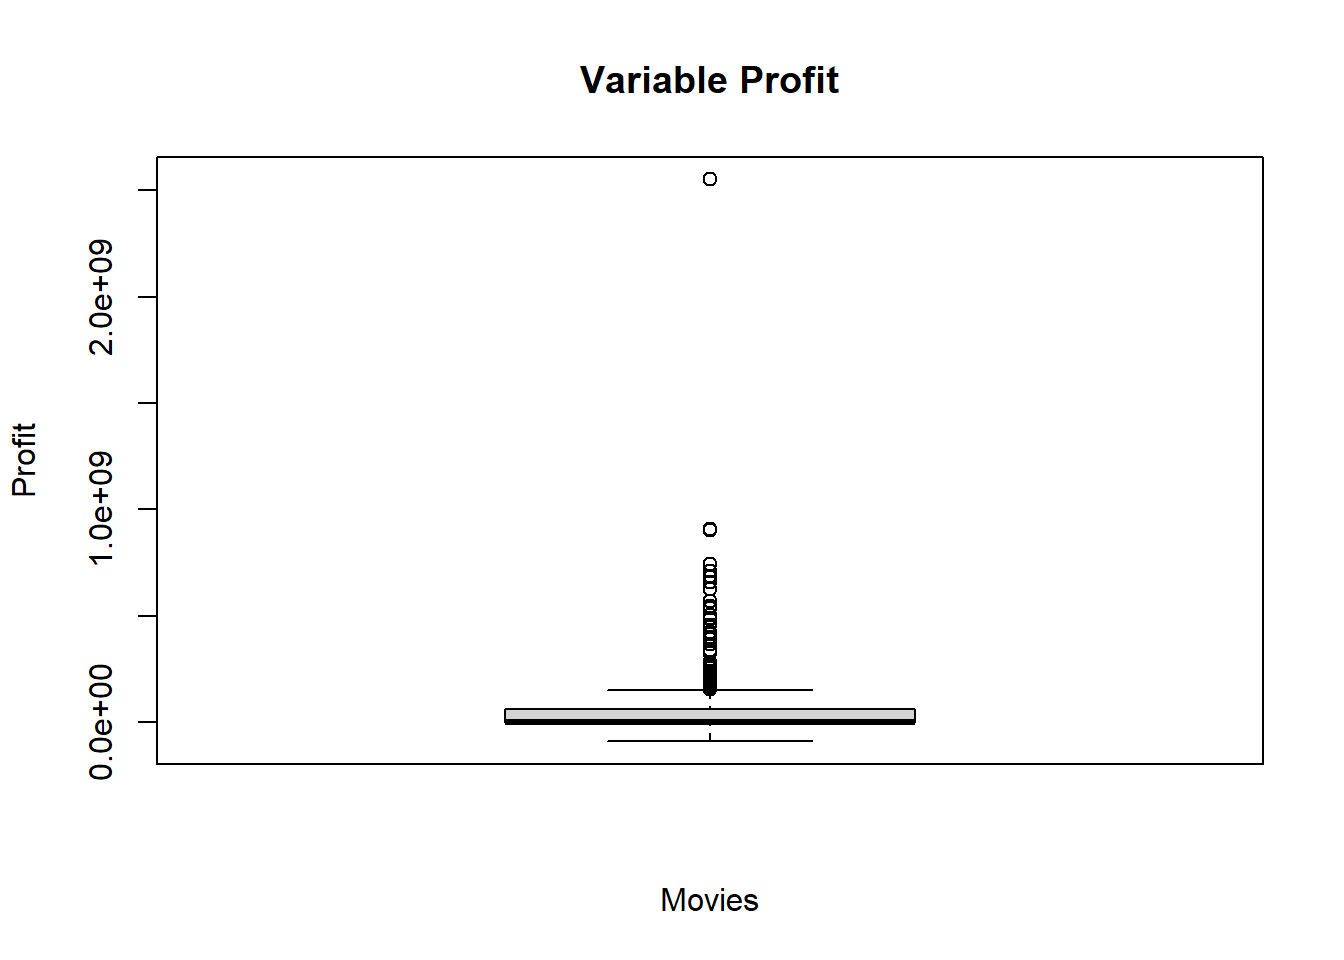
\includegraphics[keepaspectratio]{Assignment2_files/figure-latex/unnamed-chunk-5-1.pdf}}

\begin{Shaded}
\begin{Highlighting}[]
\NormalTok{movies }\SpecialCharTok{\%\textgreater{}\%}
  \FunctionTok{summarise}\NormalTok{(}\AttributeTok{Q1 =} \FunctionTok{quantile}\NormalTok{(movies}\SpecialCharTok{$}\NormalTok{profit, }\FloatTok{0.25}\NormalTok{),}
            \AttributeTok{Q2 =} \FunctionTok{quantile}\NormalTok{(movies}\SpecialCharTok{$}\NormalTok{profit, }\FloatTok{0.50}\NormalTok{),}
            \AttributeTok{Q3 =} \FunctionTok{quantile}\NormalTok{(movies}\SpecialCharTok{$}\NormalTok{profit, }\FloatTok{0.75}\NormalTok{),}
            \AttributeTok{Q4 =} \FunctionTok{max}\NormalTok{(movies}\SpecialCharTok{$}\NormalTok{profit))}
\end{Highlighting}
\end{Shaded}

\begin{verbatim}
##   Q1      Q2       Q3         Q4
## 1  0 1900000 60514050 2550965087
\end{verbatim}

\begin{Shaded}
\begin{Highlighting}[]
\FunctionTok{boxplot}\NormalTok{(movies}\SpecialCharTok{$}\NormalTok{profit,}
        \AttributeTok{main=}\StringTok{\textquotesingle{}Boxplot of Variable Profit\textquotesingle{}}\NormalTok{,}
        \AttributeTok{ylab=}\StringTok{"Profit"}\NormalTok{,}
        \AttributeTok{xlab=}\StringTok{"Movies"}\NormalTok{,}
        \AttributeTok{outline =} \ConstantTok{FALSE}\NormalTok{)}
\end{Highlighting}
\end{Shaded}

\pandocbounded{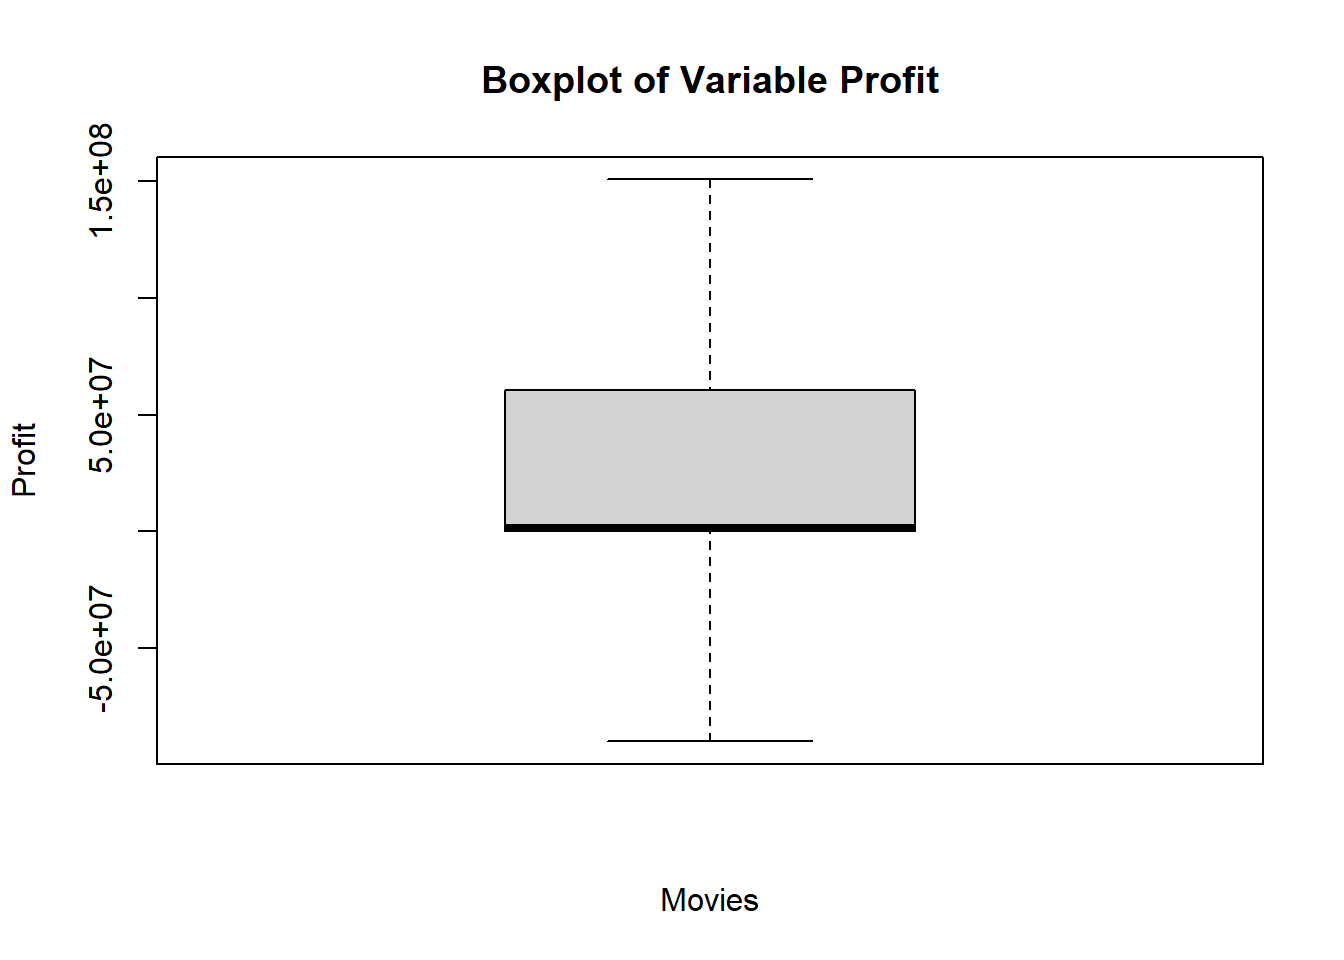
\includegraphics[keepaspectratio]{Assignment2_files/figure-latex/unnamed-chunk-5-2.pdf}}

\textbf{Your Answer:}

We created two boxplots. The first code is for all variable data in the
dataset. The resulting boxplot is very compact with many outliers. In
the second code, which was written to create the boxplot, the outliers
were removed. We did this using the line \#outline = FALSE\#. This
provides a more specific view of the distribution of variable profit.

We calculated the quantiles based on all the data, including the
outliers. These are the quantiles: Q1 = 0 Q2 = 1.900.000 Q3 = 60.514.050
Q4 = 2.550.965.087

This data tells us that the movie industry is a high-risk, high-reward
business, where the majority of films earn little, and profitability is
driven by a small fraction of massive blockbusters.

\emph{Step d}

\begin{Shaded}
\begin{Highlighting}[]
\CommentTok{\#WRITE YOUR CODE HERE}

\NormalTok{movies}\SpecialCharTok{$}\NormalTok{log\_profits }\OtherTok{=} \FunctionTok{log}\NormalTok{(movies}\SpecialCharTok{$}\NormalTok{profit)}
\end{Highlighting}
\end{Shaded}

\begin{verbatim}
## Warning in log(movies$profit): NaNs produced
\end{verbatim}

\begin{Shaded}
\begin{Highlighting}[]
\NormalTok{movies }\SpecialCharTok{\%\textgreater{}\%}
  \FunctionTok{summarise}\NormalTok{(}\AttributeTok{mean\_profits =} \FunctionTok{mean}\NormalTok{(movies}\SpecialCharTok{$}\NormalTok{log\_profits))}
\end{Highlighting}
\end{Shaded}

\begin{verbatim}
##   mean_profits
## 1          NaN
\end{verbatim}

\begin{Shaded}
\begin{Highlighting}[]
\NormalTok{movies }\SpecialCharTok{\%\textgreater{}\%}
  \FunctionTok{summarise}\NormalTok{(}\AttributeTok{mean\_profits2 =} \FunctionTok{mean}\NormalTok{(log\_profits[}\FunctionTok{is.finite}\NormalTok{(log\_profits)], }\AttributeTok{na.rm =} \ConstantTok{TRUE}\NormalTok{))}
\end{Highlighting}
\end{Shaded}

\begin{verbatim}
##   mean_profits2
## 1      17.38094
\end{verbatim}

\textbf{Your Answer:}

All films without profit are converted to -infinity, because the value
of log(0) is not defined for any base of the logarithm All films with a
negative profit are converted to NaN, which means that the result of a
mathematical calculation is not a valid number. This is because the
logarithm is only defined for positive real numbers.

As a result, when calculating the average logarithm of profits, it
returns NaN. To obtain an average, films with zero or negative profits
should be excluded from the calculation, as their logarithm values are
undefined. The average then only reflects films with positive profits.
The only problem is that this distorts the result because loss-making or
break-even films are not taken into account.

\emph{Step e}

\begin{Shaded}
\begin{Highlighting}[]
\CommentTok{\#WRITE YOUR CODE HERE}
\NormalTok{movies}\SpecialCharTok{$}\NormalTok{log\_profits[movies}\SpecialCharTok{$}\NormalTok{log\_profits}\SpecialCharTok{\textless{}=}\DecValTok{0}\NormalTok{]}\OtherTok{\textless{}{-}} \ConstantTok{NA}
\NormalTok{movies}\SpecialCharTok{$}\NormalTok{log\_profits[}\FunctionTok{is.nan}\NormalTok{(movies}\SpecialCharTok{$}\NormalTok{log\_profits)] }\OtherTok{\textless{}{-}} \ConstantTok{NA}

\FunctionTok{mean}\NormalTok{(movies}\SpecialCharTok{$}\NormalTok{log\_profits, }\AttributeTok{na.rm =} \ConstantTok{TRUE}\NormalTok{)}
\end{Highlighting}
\end{Shaded}

\begin{verbatim}
## [1] 17.38094
\end{verbatim}

\begin{Shaded}
\begin{Highlighting}[]
\FunctionTok{boxplot}\NormalTok{(movies}\SpecialCharTok{$}\NormalTok{log\_profits,}
        \AttributeTok{main =} \StringTok{"Boxplot of Variable Log(Profits)"}\NormalTok{,}
        \AttributeTok{xlab =} \StringTok{"Movies"}\NormalTok{,}
        \AttributeTok{ylab =} \StringTok{"Log of Profits"}\NormalTok{)}
\end{Highlighting}
\end{Shaded}

\pandocbounded{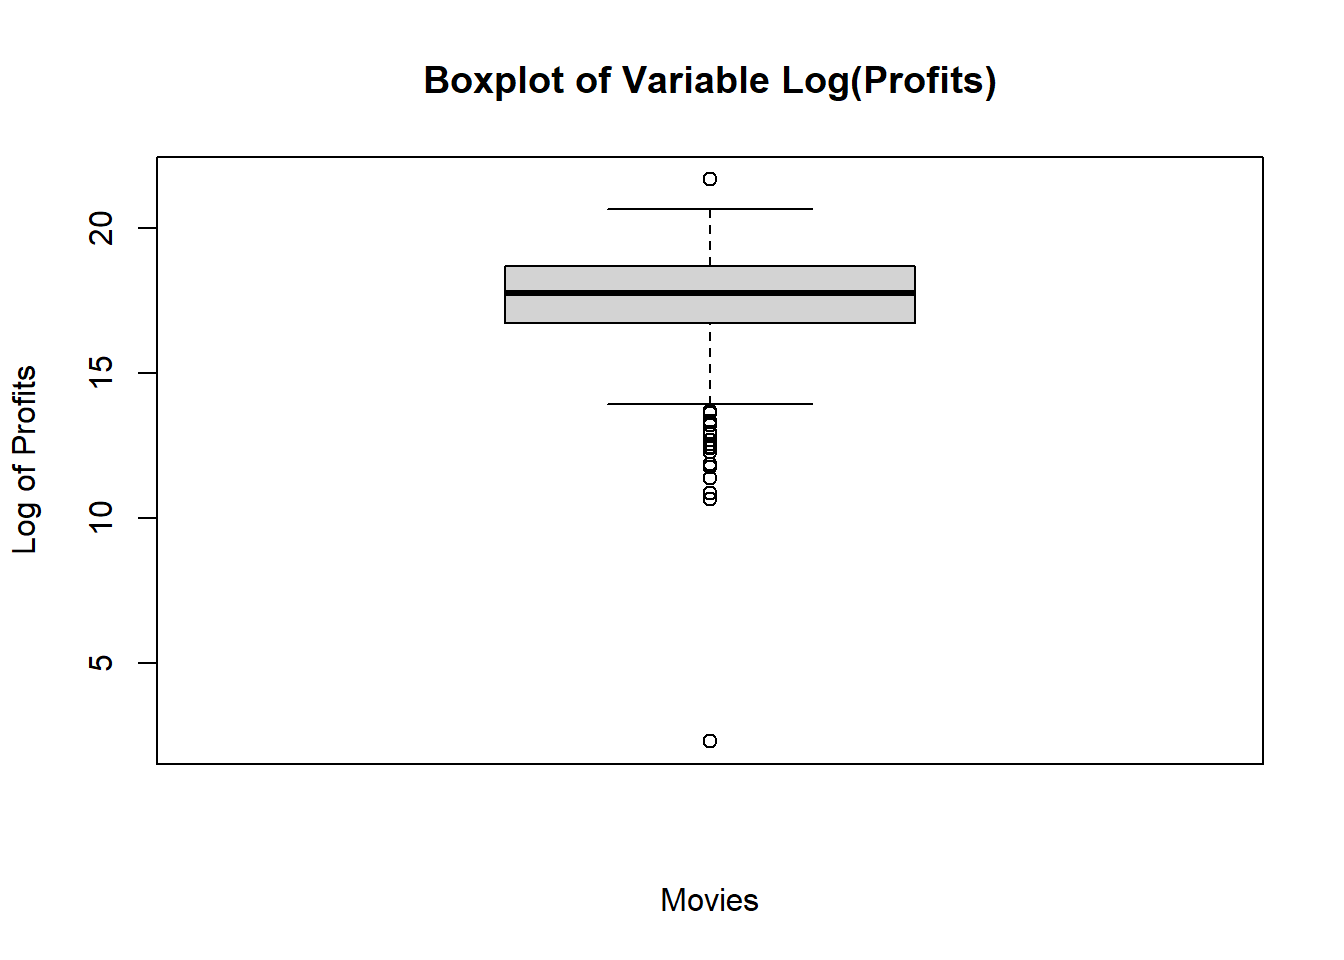
\includegraphics[keepaspectratio]{Assignment2_files/figure-latex/unnamed-chunk-7-1.pdf}}

\textbf{Your Answer:} The log scale compresses extremely large profits
and expands smaller ones, which places the values on a more manageable
scale. Therefore the boxplot provides more information than in
c.~Additionally, all negative values have been removed from the data, so
only positive values are visible in the boxplot. However, there are
still outliers, which can be seen as the points below and above the
boxplot.

\emph{Step f}

\begin{Shaded}
\begin{Highlighting}[]
\CommentTok{\#WRITE YOUR CODE HERE}
\FunctionTok{ggplot}\NormalTok{(movies, }\FunctionTok{aes}\NormalTok{(}\AttributeTok{x=}\NormalTok{runtime, }\AttributeTok{y=}\NormalTok{vote\_average))}\SpecialCharTok{+}
  \FunctionTok{geom\_point}\NormalTok{()}\SpecialCharTok{+}
  \FunctionTok{geom\_smooth}\NormalTok{(}\AttributeTok{method=}\StringTok{"lm"}\NormalTok{, }\AttributeTok{se=}\NormalTok{T)}
\end{Highlighting}
\end{Shaded}

\begin{verbatim}
## `geom_smooth()` using formula = 'y ~ x'
\end{verbatim}

\begin{verbatim}
## Warning: Removed 1 row containing non-finite outside the scale range
## (`stat_smooth()`).
\end{verbatim}

\begin{verbatim}
## Warning: Removed 1 row containing missing values or values outside the scale range
## (`geom_point()`).
\end{verbatim}

\pandocbounded{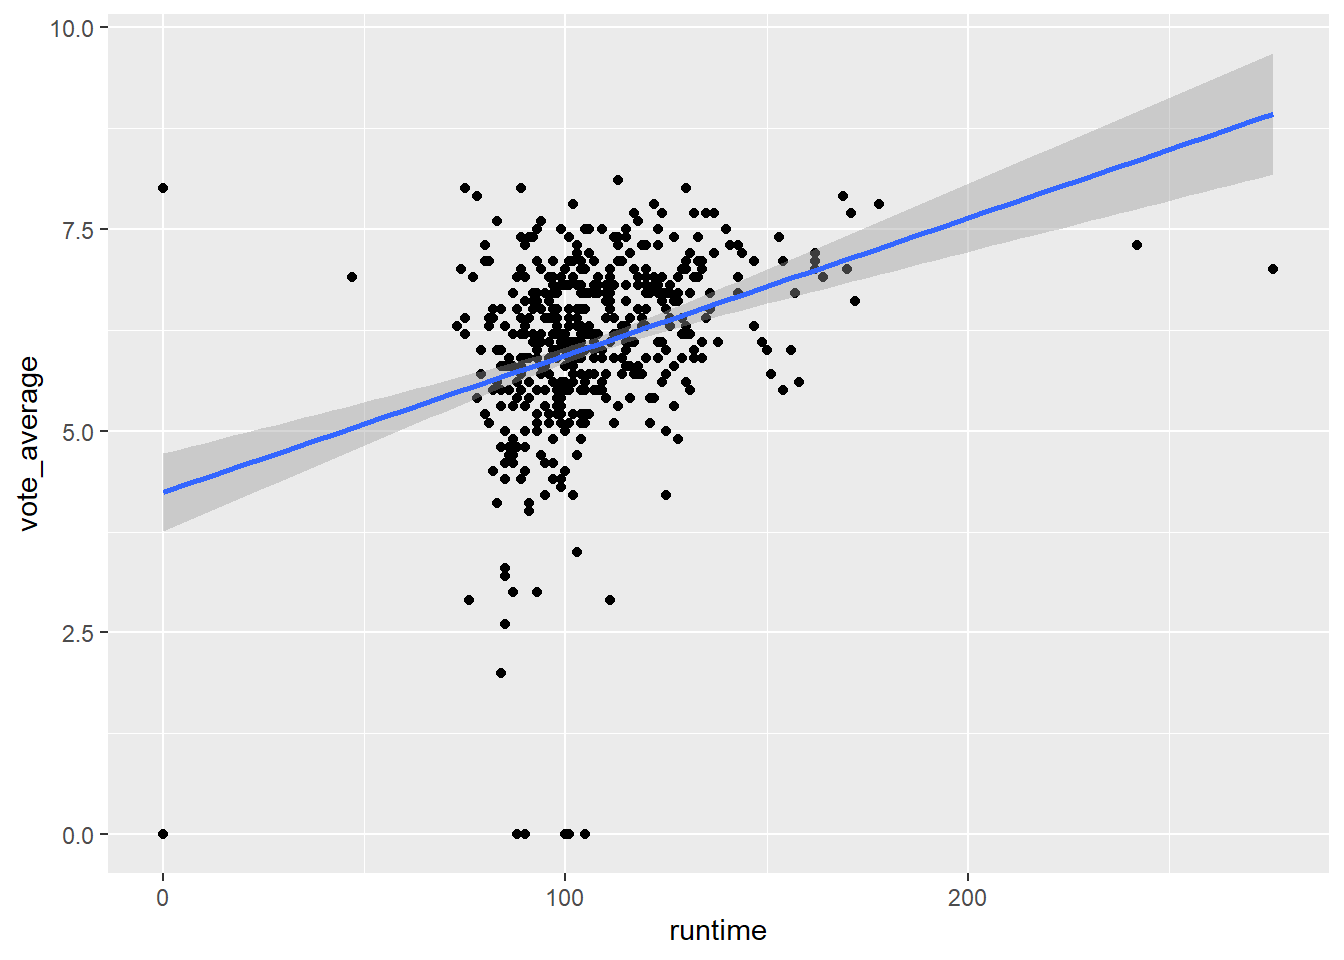
\includegraphics[keepaspectratio]{Assignment2_files/figure-latex/unnamed-chunk-8-1.pdf}}

\textbf{Your Answer:}

The average lies around the 100 minutes, movies with a longer runtime
are considered better. This suggests that viewers may perceive longer
movies as more developed or higher quality.

\section{Week 2}\label{week-2}

1 Is your dataset movies1.tsv the full population, or is it a sample of
a larger population? If the latter, how would you describe the full
population? \textbf{[4 points]}

\begin{Shaded}
\begin{Highlighting}[]
\CommentTok{\#WRITE YOUR CODE HERE}

\FunctionTok{head}\NormalTok{(movies}\SpecialCharTok{$}\NormalTok{index, }\AttributeTok{n =} \DecValTok{10}\NormalTok{)}
\end{Highlighting}
\end{Shaded}

\begin{verbatim}
##  [1] 1773 2540 1174 3262 4324  214 1737  610 2738  963
\end{verbatim}

\begin{Shaded}
\begin{Highlighting}[]
\FunctionTok{nrow}\NormalTok{(movies)}
\end{Highlighting}
\end{Shaded}

\begin{verbatim}
## [1] 505
\end{verbatim}

\textbf{Your Answer:}

These numbers are the first ten index numbers of the responders of this
data set. As you can see, many numbers are missing. This shows that this
is an sample and not an entire population. There are 505 subjects
(movies), while the index is showing there are many more. Furthermore,
you can logically reason that more than 505 films have been made
worldwide.

2 a. For which actor in your data set do you observe the most movies?
\textbf{[2 points]} b. What is the average revenue of the movie in which
this actor plays and does the revenue lie above or below the revenue of
an average movie according to your data set? \textbf{[2 points]}\\
c.~How trustworthy do you consider your conclusion to answer 2b? Use the
term ``law of large numbers'' in your explanation. \textbf{[2 points]}

\emph{step a}

\begin{Shaded}
\begin{Highlighting}[]
\CommentTok{\#WRITE YOUR CODE HERE}
\NormalTok{actor\_counts }\OtherTok{\textless{}{-}} \FunctionTok{sort}\NormalTok{(}\FunctionTok{table}\NormalTok{(movies}\SpecialCharTok{$}\NormalTok{first\_actor), }\AttributeTok{decreasing =} \ConstantTok{TRUE}\NormalTok{)}
\FunctionTok{head}\NormalTok{(actor\_counts, }\DecValTok{1}\NormalTok{)}
\end{Highlighting}
\end{Shaded}

\begin{verbatim}
## 
## Bruce Willis 
##            7
\end{verbatim}

\textbf{Your Answer:}

Bruce Willis is the actor who plays in the most movies. He plays in 7
movies.

\emph{step b}

\begin{Shaded}
\begin{Highlighting}[]
\CommentTok{\#WRITE YOUR CODE HERE}
\NormalTok{movies }\SpecialCharTok{\%\textgreater{}\%} 
  \FunctionTok{filter}\NormalTok{(first\_actor}\SpecialCharTok{==}\StringTok{"Bruce Willis"}\NormalTok{) }\SpecialCharTok{\%\textgreater{}\%} 
  \FunctionTok{summarise}\NormalTok{(}\AttributeTok{avg\_revenue\_Bruce=}\FunctionTok{mean}\NormalTok{(revenue, }\AttributeTok{na.rm=}\NormalTok{T))}
\end{Highlighting}
\end{Shaded}

\begin{verbatim}
##   avg_revenue_Bruce
## 1         116280090
\end{verbatim}

\begin{Shaded}
\begin{Highlighting}[]
\NormalTok{movies }\SpecialCharTok{\%\textgreater{}\%}
  \FunctionTok{summarise}\NormalTok{(}\AttributeTok{avg\_revenue\_data =} \FunctionTok{mean}\NormalTok{(movies}\SpecialCharTok{$}\NormalTok{revenue))}
\end{Highlighting}
\end{Shaded}

\begin{verbatim}
##   avg_revenue_data
## 1         94815482
\end{verbatim}

\textbf{Your Answer:}

The average revenue of the films of Bruce Willis is 116.280.090. The
average revenue of all the films is 94.815.482. The average revenue of
the films of Bruce Willis lies above the average revenue of all the
films.

\emph{step c}

\textbf{Your Answer:} The conclusion in 2b is not very trustworthy,
because it is based only on the subset of movies with Bruce Willis.
According to the law of large numbers, the reliability of an average
increases as the sample size grows. Since the number of Bruce Willis
films in the dataset is much smaller (7) than the total number of films
(505), his average revenue may not accurately reflect the true
expectation and could be influenced by a few exceptionally high-grossing
films.

3 For this question, you will assume that your data set is the full
population. a. Recode profits such that it is expressed in millions.
What is the variance of the variable profits (in millions) in your data
set? \textbf{[2 points]} b. Create a new data set, called
movies\_sample. Make sure that it is a random sample of your data set of
25 movies. What is the variance of profits in this random sample? How
does it compare to the variance of profits in 2a? \textbf{[2 points]}
c.~In a for loop, create 100 different samples of 25 movies, as in b,
and estimate the variance within each sample. Save the variance of each
sample in a vector called sample\_vars. So the first position of the
vector would have the variance of the first sample, the second position
the variance of the second sample, etc. Print the start of this vector.
\textbf{[2 points]} d.~Summarize and make a histogram of sample\_vars.
What is the mean, standard deviation and shape of its distribution?
\textbf{[2 points]} e. In your opinion, is a sample of 25 movies
sufficient to get a reliable estimate of the population variance of
profits, using the sample variance? Explain? \textbf{[2 points]}

\emph{step a}

\begin{Shaded}
\begin{Highlighting}[]
\CommentTok{\#WRITE YOUR CODE HERE}

\NormalTok{movies}\SpecialCharTok{$}\NormalTok{profit }\OtherTok{=}\NormalTok{ movies}\SpecialCharTok{$}\NormalTok{profit}\SpecialCharTok{/}\DecValTok{1000000}
\NormalTok{variance }\OtherTok{=} \FunctionTok{var}\NormalTok{(movies}\SpecialCharTok{$}\NormalTok{profit)}
\end{Highlighting}
\end{Shaded}

\textbf{Your Answer:}

The variance of of the variable profits (in millions) is 30463,13

\emph{step b}

\begin{Shaded}
\begin{Highlighting}[]
\CommentTok{\#WRITE YOUR CODE HERE}

\FunctionTok{set.seed}\NormalTok{(}\DecValTok{123}\NormalTok{)}

\NormalTok{movies\_sample }\OtherTok{\textless{}{-}}\NormalTok{ movies[}\FunctionTok{sample}\NormalTok{(}\FunctionTok{nrow}\NormalTok{(movies), }\DecValTok{25}\NormalTok{), ]}
\NormalTok{variance\_sample }\OtherTok{=} \FunctionTok{var}\NormalTok{(movies\_sample}\SpecialCharTok{$}\NormalTok{profit)}
\end{Highlighting}
\end{Shaded}

\textbf{Your Answer:}

The variance of profits in the sample of 25 movies is 5156 million,
which is much lower than the variance of the full dataset. When we
computed a sample multiple times, we saw a lot of changes in the
variance. Sometimes there were no outliers which made the variance very
low, but sometimes the variance was higher than the population variance.
Normally we would expect the population variance to be lower, because it
it a more precise variable. But in this case the sample chooses movies
with less/no outliers, causing the variable to be lower.

\emph{step c}

\begin{Shaded}
\begin{Highlighting}[]
\CommentTok{\#WRITE YOUR CODE HERE}

\FunctionTok{library}\NormalTok{(dplyr)}

\FunctionTok{set.seed}\NormalTok{(}\DecValTok{123}\NormalTok{)}

\NormalTok{sample\_vars }\OtherTok{\textless{}{-}} \FunctionTok{c}\NormalTok{()}
\ControlFlowTok{for}\NormalTok{ (i }\ControlFlowTok{in} \DecValTok{1}\SpecialCharTok{:}\DecValTok{100}\NormalTok{) \{}
\NormalTok{  sample\_data }\OtherTok{\textless{}{-}} \FunctionTok{sample}\NormalTok{(movies}\SpecialCharTok{$}\NormalTok{profit, }\AttributeTok{size =} \DecValTok{25}\NormalTok{, }\AttributeTok{replace =} \ConstantTok{TRUE}\NormalTok{)}
\NormalTok{  sample\_vars[i] }\OtherTok{\textless{}{-}} \FunctionTok{var}\NormalTok{(sample\_data)}
\NormalTok{\}}

\FunctionTok{print}\NormalTok{(sample\_vars)}
\end{Highlighting}
\end{Shaded}

\begin{verbatim}
##   [1]   5427.987   2599.269   1786.823   4188.200  19863.914   2262.348
##   [7]   3726.957  14556.274  21766.930   6832.605   1087.340  65016.009
##  [13]  47405.135  26631.279  30006.369  24206.674  36152.296   8018.320
##  [19]  49524.980   3851.321  20117.246  26119.756  23950.476  10173.782
##  [25]  36207.858  10970.705   1781.194  19492.944  34422.145  18251.876
##  [31]   2517.222   5662.617  13437.085  18254.151   1927.698  21495.217
##  [37]   1199.210  11642.164   1076.289  20104.961  16522.001  13616.902
##  [43] 259978.030   2494.030   5680.998  23620.087  21488.611  27307.159
##  [49]  39659.398  10125.730  41241.568  34881.842  42593.662  30249.814
##  [55]  11788.002   2526.887   8144.473   3685.787  14342.990  20354.465
##  [61]  10290.612  27415.819   9400.046   7981.578  25090.506  16657.474
##  [67]  36231.807   4069.141  14573.631  11745.178  17524.721  10498.433
##  [73]   2284.862  11283.803  40114.139 263450.409   4958.309  11272.150
##  [79]  12774.466   8603.828  23926.725   7253.008  14657.673  25011.299
##  [85]  30413.328  11457.522  10852.733  33606.377  60474.045  41136.172
##  [91]  10983.993   2295.091  13451.089   8751.209  16105.003   7259.011
##  [97]  29709.776  14968.661  27246.490  34187.963
\end{verbatim}

\textbf{Your Answer:}

Above are the profit variances of 100 different samples.

\emph{step d}

\begin{Shaded}
\begin{Highlighting}[]
\CommentTok{\#WRITE YOUR CODE HERE}
\NormalTok{dfsample\_vars }\OtherTok{=} \FunctionTok{as.data.frame}\NormalTok{(sample\_vars)}

\FunctionTok{ggplot}\NormalTok{(dfsample\_vars, }\FunctionTok{aes}\NormalTok{(}\AttributeTok{x =}\NormalTok{ sample\_vars)) }\SpecialCharTok{+}
  \FunctionTok{geom\_histogram}\NormalTok{(}\AttributeTok{bins =} \DecValTok{50}\NormalTok{) }\SpecialCharTok{+}
  \FunctionTok{labs}\NormalTok{(}\AttributeTok{title =} \StringTok{"Histogram of sample variances"}\NormalTok{, }\AttributeTok{x =} \StringTok{"Sample variances"}\NormalTok{, }\AttributeTok{y =} \StringTok{"Frequency"}\NormalTok{)}
\end{Highlighting}
\end{Shaded}

\pandocbounded{\includegraphics[keepaspectratio]{Assignment2_files/figure-latex/unnamed-chunk-15-1.pdf}}

\begin{Shaded}
\begin{Highlighting}[]
\NormalTok{dfsample\_vars }\SpecialCharTok{\%\textgreater{}\%}
  \FunctionTok{summarise}\NormalTok{(}\AttributeTok{mean\_sample =} \FunctionTok{mean}\NormalTok{(sample\_vars),}
            \AttributeTok{sd\_sample =} \FunctionTok{sd}\NormalTok{(sample\_vars))}
\end{Highlighting}
\end{Shaded}

\begin{verbatim}
##   mean_sample sd_sample
## 1    22739.86  36935.63
\end{verbatim}

\begin{Shaded}
\begin{Highlighting}[]
\FunctionTok{library}\NormalTok{(e1071)}
\end{Highlighting}
\end{Shaded}

\begin{verbatim}
## Warning: package 'e1071' was built under R version 4.5.1
\end{verbatim}

\begin{Shaded}
\begin{Highlighting}[]
\NormalTok{skewness\_sample }\OtherTok{=} \FunctionTok{skewness}\NormalTok{(sample\_vars, }\AttributeTok{na.rm=}\NormalTok{T)}
\NormalTok{kurtosis\_sample }\OtherTok{=} \FunctionTok{kurtosis}\NormalTok{(sample\_vars, }\AttributeTok{na.rm=}\NormalTok{T)}
\FunctionTok{print}\NormalTok{(skewness\_sample)}
\end{Highlighting}
\end{Shaded}

\begin{verbatim}
## [1] 5.414064
\end{verbatim}

\begin{Shaded}
\begin{Highlighting}[]
\FunctionTok{print}\NormalTok{(kurtosis\_sample)}
\end{Highlighting}
\end{Shaded}

\begin{verbatim}
## [1] 32.11739
\end{verbatim}

\textbf{Your Answer:}

The mean of the sample variances is 22739,86. The standard deviation of
the sample variances is 36935,63. The shape of the distribution is
right-skewed, because of the positive skewness value. The kurtosis value
is very high, because of the heavy outlier.

\emph{step e}

\textbf{Your Answer:}

A sample of 25 movies is relatively small for estimating the population
variance of profits. The variance is very sensitive to extreme values,
and as seen in the histogram, movie profits are highly skewed with large
outliers. According to the law of large numbers, larger samples are
needed for the sample variance to converge to the true population
variance.

\textbf{Your answer here}

\section{Week 3}\label{week-3}

For the next part of the assignment, assume that the movies in your data
frame are a random sample of a larger population of movies.

1 a. Create a new data set that only includes movies that are of the
genre ``Thriller''. For these thriller movies, give a 99 percent
confidence interval for the variable \emph{runtime}. Interpret the
result. \textbf{[2 points]} b. Now, assume that the variance of
\emph{runtime} amongst thriller movies in your data is exactly the same
as the variance of \emph{runtime} in the population. Under this
assumption, give a 99 percent confidence interval for the variable
\emph{runtime} among thriller movies. Interpret the result. Is you
confidence interval wider or less wide than the one you found under
question 1a? Why is that the case? \textbf{[2 points]}

\emph{step a}

\begin{Shaded}
\begin{Highlighting}[]
\CommentTok{\#WRITE YOUR CODE HERE}

\NormalTok{thriller\_movies }\OtherTok{\textless{}{-}} \FunctionTok{subset}\NormalTok{(movies, }\FunctionTok{grepl}\NormalTok{(}\StringTok{"Thriller"}\NormalTok{, genre, }\AttributeTok{ignore.case =} \ConstantTok{FALSE}\NormalTok{))}

\NormalTok{t\_result }\OtherTok{=} \FunctionTok{t.test}\NormalTok{(thriller\_movies}\SpecialCharTok{$}\NormalTok{runtime, }\AttributeTok{conf.level =} \FloatTok{0.99}\NormalTok{)}
\NormalTok{conf\_interval }\OtherTok{=}\NormalTok{ t\_result}\SpecialCharTok{$}\NormalTok{conf.int}
\FunctionTok{print}\NormalTok{(conf\_interval)}
\end{Highlighting}
\end{Shaded}

\begin{verbatim}
## [1]  99.94343 111.01042
## attr(,"conf.level")
## [1] 0.99
\end{verbatim}

\textbf{Your Answer:}

We are 99\% confident that the true mean runtime of all thriller movies
in the population falls between 99.94 and 111.01 minutes.

\emph{step b}

\begin{Shaded}
\begin{Highlighting}[]
\CommentTok{\#WRITE YOUR CODE HERE}

\NormalTok{mean\_runtime }\OtherTok{=} \FunctionTok{mean}\NormalTok{(thriller\_movies}\SpecialCharTok{$}\NormalTok{runtime)}
\NormalTok{sd\_runtime }\OtherTok{=} \FunctionTok{sd}\NormalTok{(thriller\_movies}\SpecialCharTok{$}\NormalTok{runtime)}
\NormalTok{n }\OtherTok{=} \FunctionTok{length}\NormalTok{(thriller\_movies}\SpecialCharTok{$}\NormalTok{runtime)}

\NormalTok{sd\_population }\OtherTok{=}\NormalTok{ sd\_runtime}

\NormalTok{alpha }\OtherTok{\textless{}{-}} \FloatTok{0.01}
\NormalTok{z }\OtherTok{=} \FunctionTok{qnorm}\NormalTok{(}\DecValTok{1}\SpecialCharTok{{-}}\NormalTok{alpha}\SpecialCharTok{/}\DecValTok{2}\NormalTok{)}
\NormalTok{error\_margin }\OtherTok{=}\NormalTok{ z}\SpecialCharTok{*}\NormalTok{(sd\_population}\SpecialCharTok{/}\FunctionTok{sqrt}\NormalTok{(n))}
\NormalTok{LOW }\OtherTok{=}\NormalTok{ mean\_runtime }\SpecialCharTok{{-}}\NormalTok{ error\_margin}
\NormalTok{UP }\OtherTok{=}\NormalTok{ mean\_runtime }\SpecialCharTok{+}\NormalTok{ error\_margin}

\FunctionTok{print}\NormalTok{(}\FunctionTok{c}\NormalTok{(LOW, UP))}
\end{Highlighting}
\end{Shaded}

\begin{verbatim}
## [1] 100.1081 110.8457
\end{verbatim}

\textbf{Your Answer:}

We are 99\% confident that the true mean runtime of thriller movies in
the entire population falls between 100.11 and 110.85 minutes.

2 a. Using an appropriate five-step procedure, set up a test for the
null hypothesis that the variance of runtime equals \(500\). Clearly
state your null hypothesis, alternative hypothesis your test statistic,
your critical value, and your conclusion. \textbf{[2 points]} b. For the
validity of your test in 2a, what assumption about the distribution of
revenue needs to hold? Make an appropriate plot to test this assumption.
What do you conclude? \textbf{[2 points]}

\emph{step a}

\begin{Shaded}
\begin{Highlighting}[]
\CommentTok{\#WRITE YOUR CODE HERE}
\NormalTok{s2 }\OtherTok{=} \FunctionTok{var}\NormalTok{(movies}\SpecialCharTok{$}\NormalTok{runtime, }\AttributeTok{na.rm =} \ConstantTok{TRUE}\NormalTok{)}
\NormalTok{n }\OtherTok{=} \FunctionTok{sum}\NormalTok{(}\SpecialCharTok{!}\FunctionTok{is.na}\NormalTok{(movies}\SpecialCharTok{$}\NormalTok{runtime))}

\CommentTok{\# Hypothesized variance}
\NormalTok{sigma2 }\OtherTok{\textless{}{-}} \DecValTok{500}

\CommentTok{\# Test statistic}
\NormalTok{test\_statistic }\OtherTok{\textless{}{-}}\NormalTok{ (n }\SpecialCharTok{{-}} \DecValTok{1}\NormalTok{) }\SpecialCharTok{*}\NormalTok{ s2 }\SpecialCharTok{/}\NormalTok{ sigma2}

\CommentTok{\# Print test statistic}
\FunctionTok{cat}\NormalTok{(}\StringTok{"test statistic:"}\NormalTok{, }\FunctionTok{round}\NormalTok{(test\_statistic, }\DecValTok{2}\NormalTok{), }\StringTok{"}\SpecialCharTok{\textbackslash{}n}\StringTok{"}\NormalTok{)}
\end{Highlighting}
\end{Shaded}

\begin{verbatim}
## test statistic: 486
\end{verbatim}

\begin{Shaded}
\begin{Highlighting}[]
\CommentTok{\#critical value}
\NormalTok{alpha2 }\OtherTok{\textless{}{-}} \FloatTok{0.05}
\NormalTok{lower }\OtherTok{\textless{}{-}} \FunctionTok{qchisq}\NormalTok{(alpha }\SpecialCharTok{/} \DecValTok{2}\NormalTok{, }\AttributeTok{df =}\NormalTok{ n }\SpecialCharTok{{-}} \DecValTok{1}\NormalTok{)}
\NormalTok{upper }\OtherTok{\textless{}{-}} \FunctionTok{qchisq}\NormalTok{(}\DecValTok{1} \SpecialCharTok{{-}}\NormalTok{ alpha }\SpecialCharTok{/} \DecValTok{2}\NormalTok{, }\AttributeTok{df =}\NormalTok{ n }\SpecialCharTok{{-}} \DecValTok{1}\NormalTok{)}

\CommentTok{\#print}
\FunctionTok{cat}\NormalTok{(}\StringTok{"Critical values:}\SpecialCharTok{\textbackslash{}n}\StringTok{"}\NormalTok{)}
\end{Highlighting}
\end{Shaded}

\begin{verbatim}
## Critical values:
\end{verbatim}

\begin{Shaded}
\begin{Highlighting}[]
\FunctionTok{cat}\NormalTok{(}\StringTok{"Lower:"}\NormalTok{, }\FunctionTok{round}\NormalTok{(lower, }\DecValTok{2}\NormalTok{), }\StringTok{"}\SpecialCharTok{\textbackslash{}n}\StringTok{"}\NormalTok{)}
\end{Highlighting}
\end{Shaded}

\begin{verbatim}
## Lower: 425.06
\end{verbatim}

\begin{Shaded}
\begin{Highlighting}[]
\FunctionTok{cat}\NormalTok{(}\StringTok{"Upper:"}\NormalTok{, }\FunctionTok{round}\NormalTok{(upper, }\DecValTok{2}\NormalTok{), }\StringTok{"}\SpecialCharTok{\textbackslash{}n}\StringTok{"}\NormalTok{)}
\end{Highlighting}
\end{Shaded}

\begin{verbatim}
## Upper: 588.45
\end{verbatim}

\begin{Shaded}
\begin{Highlighting}[]
\CommentTok{\#compare test statistic with the critical}
\ControlFlowTok{if}\NormalTok{ (test\_statistic }\SpecialCharTok{\textless{}}\NormalTok{ lower }\SpecialCharTok{||}\NormalTok{ test\_statistic }\SpecialCharTok{\textgreater{}}\NormalTok{ upper) \{}
  \FunctionTok{cat}\NormalTok{(}\StringTok{"Reject the null hypothesis.}\SpecialCharTok{\textbackslash{}n}\StringTok{"}\NormalTok{)}
\NormalTok{\} }\ControlFlowTok{else}\NormalTok{ \{}
  \FunctionTok{cat}\NormalTok{(}\StringTok{"Do not reject the null hypothesis.}\SpecialCharTok{\textbackslash{}n}\StringTok{"}\NormalTok{)}
\NormalTok{\}}
\end{Highlighting}
\end{Shaded}

\begin{verbatim}
## Do not reject the null hypothesis.
\end{verbatim}

\textbf{Your Answer:}

The null hypothesis (H0) is equal to 500. The alternative hypothesis
(H1) is NOT equal to 500. We computed the test statistic and the
critical values. Our conclusion is that we do not reject the null
hypothesis.

\emph{step b}

\begin{Shaded}
\begin{Highlighting}[]
\CommentTok{\#WRITE YOUR CODE HERE}
\FunctionTok{ggplot}\NormalTok{(movies, }\FunctionTok{aes}\NormalTok{(}\AttributeTok{x =}\NormalTok{ runtime))}\SpecialCharTok{+}
  \FunctionTok{geom\_histogram}\NormalTok{()}\SpecialCharTok{+}
  \FunctionTok{labs}\NormalTok{(}\AttributeTok{title =} \StringTok{"Histogram of runtime"}\NormalTok{,}
       \AttributeTok{y =} \StringTok{"frequency"}\NormalTok{)}
\end{Highlighting}
\end{Shaded}

\begin{verbatim}
## `stat_bin()` using `bins = 30`. Pick better value with `binwidth`.
\end{verbatim}

\begin{verbatim}
## Warning: Removed 1 row containing non-finite outside the scale range
## (`stat_bin()`).
\end{verbatim}

\pandocbounded{\includegraphics[keepaspectratio]{Assignment2_files/figure-latex/unnamed-chunk-19-1.pdf}}

\begin{Shaded}
\begin{Highlighting}[]
\FunctionTok{ggplot}\NormalTok{(movies, }\FunctionTok{aes}\NormalTok{(}\AttributeTok{sample =}\NormalTok{ runtime)) }\SpecialCharTok{+}
  \FunctionTok{stat\_qq}\NormalTok{() }\SpecialCharTok{+}
  \FunctionTok{stat\_qq\_line}\NormalTok{(}\AttributeTok{color =} \StringTok{"purple"}\NormalTok{) }\SpecialCharTok{+}
  \FunctionTok{labs}\NormalTok{(}\AttributeTok{title =} \StringTok{"Normal QQ plot"}\NormalTok{,}
       \AttributeTok{x =} \StringTok{"Theoretical Quantiles"}\NormalTok{,}
       \AttributeTok{y =} \StringTok{"Sample Quantilies"}\NormalTok{) }\SpecialCharTok{+}
  \FunctionTok{theme\_minimal}\NormalTok{()}
\end{Highlighting}
\end{Shaded}

\begin{verbatim}
## Warning: Removed 1 row containing non-finite outside the scale range
## (`stat_qq()`).
\end{verbatim}

\begin{verbatim}
## Warning: Removed 1 row containing non-finite outside the scale range
## (`stat_qq_line()`).
\end{verbatim}

\pandocbounded{\includegraphics[keepaspectratio]{Assignment2_files/figure-latex/unnamed-chunk-19-2.pdf}}

\textbf{Your Answer:}

*I think there is a typo in question 2b, because for 2a we are doing
hypothesis testing for the runtime. It would be weird to reason about
assumptions of revenue, which has nothing to do with the runtime.

The assumption for the chi-square variance test is that the runtime
variable is normally distributed. The histogram of runtime shows a
concentration around 90--120 minutes, but the distribution is slightly
right-skewed and has a few extreme outliers at both short and very long
runtimes. The Q-Q plot also shows clear deviations from the diagonal
line, especially in the tails: very short and very long movies fall far
from what would be expected under normality Together, these plots
indicate that runtime is not perfectly normally distributed. Therefore
the normality assumption does not hold, and the result of the variance
test should be interpreted with caution.

\begin{enumerate}
\def\labelenumi{\arabic{enumi}.}
\setcounter{enumi}{2}
\tightlist
\item
  There is an argument going on in the movie studio. \emph{Bob} claims
  that they should make higher-quality movies, as this will bring in
  more profits. \emph{Chantal} disagrees. She tells Bob that mediocre
  movies bring in the most profits. You are asked to advise on who is
  right.
\end{enumerate}

\begin{enumerate}
\def\labelenumi{\alph{enumi}.}
\tightlist
\item
  Create a new variable called vote\_average\_rounded. Make sure this
  variable is the same as vote\_average, but without any decimals (i.e.,
  a 6.3 becomes a 6, a 8.7 an 8, etc.). Display a histogram of
  vote\_average\_rounded. \textbf{[2 points]}
\item
  Create a scatter plot with vote\_average\_rounded on the x axis and
  the mean of profits within each category of vote\_average\_rounded on
  the y-axis. Make sure it has an appropriate title, and appropriate
  titles and labels for the x- and y-axis. At which rating of movies are
  profits the highest? \textbf{[3 points]}
\item
  Recreate the scatter plot with year on the x axis and mean\_profits on
  the y-axis, but now add bars around each point, indicating the 95\%
  confidence interval. \textbf{[3 points]}
\item
  Write an advice to settle the argument between Bob and Chantal.
  \textbf{[4 points]}
\end{enumerate}

\emph{step a}

\begin{Shaded}
\begin{Highlighting}[]
\CommentTok{\#WRITE YOUR CODE HERE}
\NormalTok{movies}\SpecialCharTok{$}\NormalTok{vote\_average\_rounded }\OtherTok{\textless{}{-}} \FunctionTok{floor}\NormalTok{(movies}\SpecialCharTok{$}\NormalTok{vote\_average)}

\FunctionTok{ggplot}\NormalTok{(movies, }\FunctionTok{aes}\NormalTok{(}\AttributeTok{x =}\NormalTok{ vote\_average\_rounded)) }\SpecialCharTok{+}
  \FunctionTok{geom\_histogram}\NormalTok{(}\AttributeTok{binwidth =} \DecValTok{1}\NormalTok{) }\SpecialCharTok{+}
  \FunctionTok{scale\_x\_continuous}\NormalTok{(}\AttributeTok{breaks =} \FunctionTok{seq}\NormalTok{(}\DecValTok{0}\NormalTok{,}\DecValTok{8}\NormalTok{, }\AttributeTok{by =} \DecValTok{1}\NormalTok{)) }\SpecialCharTok{+}
  \FunctionTok{labs}\NormalTok{(}\AttributeTok{title =} \StringTok{"Histogram of Rounded Vote Averages"}\NormalTok{,}
       \AttributeTok{x =} \StringTok{"Vote Average"}\NormalTok{,}
       \AttributeTok{y =} \StringTok{"Frequency"}\NormalTok{) }
\end{Highlighting}
\end{Shaded}

\pandocbounded{\includegraphics[keepaspectratio]{Assignment2_files/figure-latex/unnamed-chunk-20-1.pdf}}

\textbf{Your Answer:}

With this code you create the new variable and a histogram.

\emph{step b}

\begin{Shaded}
\begin{Highlighting}[]
\CommentTok{\#WRITE YOUR CODE HERE}
\NormalTok{profit\_movies }\OtherTok{\textless{}{-}}\NormalTok{ movies }\SpecialCharTok{\%\textgreater{}\%}
  \FunctionTok{group\_by}\NormalTok{(vote\_average\_rounded) }\SpecialCharTok{\%\textgreater{}\%}
  \FunctionTok{summarise}\NormalTok{(}\AttributeTok{profit\_mean =} \FunctionTok{mean}\NormalTok{(profit, }\AttributeTok{na.rm =} \ConstantTok{TRUE}\NormalTok{))}


\FunctionTok{ggplot}\NormalTok{(profit\_movies, }\FunctionTok{aes}\NormalTok{(}\AttributeTok{x =}\NormalTok{ vote\_average\_rounded, }\AttributeTok{y =}\NormalTok{ profit\_mean)) }\SpecialCharTok{+}
  \FunctionTok{geom\_point}\NormalTok{(}\AttributeTok{size =} \DecValTok{3}\NormalTok{) }\SpecialCharTok{+}
  \FunctionTok{geom\_line}\NormalTok{() }\SpecialCharTok{+}
  \FunctionTok{labs}\NormalTok{(}
    \AttributeTok{title =} \StringTok{"Average Profit by Rounded Vote Average"}\NormalTok{,}
    \AttributeTok{x =} \StringTok{"Rounded Vote Average"}\NormalTok{,}
    \AttributeTok{y =} \StringTok{"Average Profit (in millions)"}
\NormalTok{  ) }
\end{Highlighting}
\end{Shaded}

\pandocbounded{\includegraphics[keepaspectratio]{Assignment2_files/figure-latex/unnamed-chunk-21-1.pdf}}

\textbf{Your Answer:}

The profits are the highest by a rating of 8.

\emph{step c}

\begin{Shaded}
\begin{Highlighting}[]
\CommentTok{\#WRITE YOUR CODE HERE}

\NormalTok{profit\_by\_year }\OtherTok{\textless{}{-}}\NormalTok{ movies }\SpecialCharTok{\%\textgreater{}\%}
  \FunctionTok{group\_by}\NormalTok{(release\_year) }\SpecialCharTok{\%\textgreater{}\%}
  \FunctionTok{summarise}\NormalTok{(}
    \AttributeTok{profit\_mean =} \FunctionTok{mean}\NormalTok{(profit, }\AttributeTok{na.rm =} \ConstantTok{TRUE}\NormalTok{),}
    \AttributeTok{sd =} \FunctionTok{sd}\NormalTok{(profit, }\AttributeTok{na.rm =} \ConstantTok{TRUE}\NormalTok{),}
    \AttributeTok{n =} \FunctionTok{n}\NormalTok{(),}
    \AttributeTok{se =}\NormalTok{ sd }\SpecialCharTok{/} \FunctionTok{sqrt}\NormalTok{(n),}
    \AttributeTok{lower =}\NormalTok{ profit\_mean }\SpecialCharTok{{-}} \FloatTok{1.96} \SpecialCharTok{*}\NormalTok{ se,}
    \AttributeTok{upper =}\NormalTok{ profit\_mean }\SpecialCharTok{+} \FloatTok{1.96} \SpecialCharTok{*}\NormalTok{ se}
\NormalTok{  )}

\FunctionTok{ggplot}\NormalTok{(profit\_by\_year, }\FunctionTok{aes}\NormalTok{(}\AttributeTok{x =}\NormalTok{ release\_year, }\AttributeTok{y =}\NormalTok{ profit\_mean)) }\SpecialCharTok{+}
  \FunctionTok{geom\_point}\NormalTok{(}\AttributeTok{size =} \DecValTok{2}\NormalTok{, }\AttributeTok{color =} \StringTok{"darkblue"}\NormalTok{) }\SpecialCharTok{+}
  \FunctionTok{geom\_errorbar}\NormalTok{(}\FunctionTok{aes}\NormalTok{(}\AttributeTok{ymin =}\NormalTok{ lower, }\AttributeTok{ymax =}\NormalTok{ upper), }\AttributeTok{width =} \FloatTok{0.3}\NormalTok{, }\AttributeTok{color =} \StringTok{"darkblue"}\NormalTok{) }\SpecialCharTok{+}
  \FunctionTok{labs}\NormalTok{(}
    \AttributeTok{title =} \StringTok{"Average Profit per Year (95\% Confidence Interval)"}\NormalTok{,}
    \AttributeTok{x =} \StringTok{"Release Year"}\NormalTok{,}
    \AttributeTok{y =} \StringTok{"Average Profit"}
\NormalTok{  ) }\SpecialCharTok{+}
  \FunctionTok{theme\_minimal}\NormalTok{()}
\end{Highlighting}
\end{Shaded}

\pandocbounded{\includegraphics[keepaspectratio]{Assignment2_files/figure-latex/unnamed-chunk-22-1.pdf}}

\textbf{Your Answer:}

Above you see the scatterplot created, with the 95\% confident interval.
We are not sure if it is a typo that we now have to compare the mean
profit to the release year, because it is not relevant information for
our dilemma.

\emph{step d}

\textbf{Your Answer:}

The plot shows that average profits rise with higher vote averages,
peaking at ratings around 8. This supports Bob's claim that
higher-quality movies tend to be more profitable, rather than Chantal's
view that mediocre films bring in the most profit. The yearly profit
plot shows high variation and wide confidence intervals, suggesting that
other factors like market conditions and economic environment also
matter. Still, overall the evidence favors Bob, primarily based on the
scatterplot of question b.

\end{document}
